\documentclass[11pt,a4paper]{article}

\usepackage[a4paper,margin=2.2cm,top=2.1cm,bottom=2.3cm]{geometry}
\usepackage[T1]{fontenc}
\usepackage[utf8]{inputenc}
\usepackage{mathptmx}
\usepackage{amsmath,amssymb}
\usepackage{graphicx}
\usepackage{booktabs}
\usepackage{multirow}
\usepackage{caption}
\usepackage{microtype}
\usepackage{enumitem}
\usepackage[hidelinks]{hyperref}

\captionsetup{font=small,labelfont=bf,skip=4pt}
\setlist{itemsep=1pt,topsep=3pt,parsep=0pt}
\setlength{\parskip}{2pt}

\usepackage{titlesec}
\titlespacing*{\section}{0pt}{10pt plus 2pt minus 2pt}{5pt}
\titlespacing*{\subsection}{0pt}{8pt plus 2pt minus 2pt}{4pt}
\titleformat{\section}{\large\bfseries}{\thesection.}{0.6em}{}
\titleformat{\subsection}{\normalsize\bfseries}{\thesubsection.}{0.6em}{}

\hypersetup{pdftitle={Fronthaul Load Management in Split Radio Access Networks: Benchmarking Classical and Learned Matrix Inversion for Slot-Level Compute Budgeting},
pdfauthor={Harshvardhan Choudhary (230002027), Mayank Yadav (230002041)},
pdfsubject={B.Tech. Project - Mid-Semester Evaluation Report, IIT Indore, September 2026}}

\begin{document}

% ===================== TITLE PAGE =====================
\begin{titlepage}
\centering
\vspace*{1.2cm}
{\LARGE\bfseries Fronthaul Load Management in Split Radio Access Networks: Benchmarking Classical and Learned Matrix Inversion for Slot-Level Compute Budgeting\par}
\vspace{1.6cm}
{\large B.Tech.\ Project --- Mid-Semester Evaluation Report\par}
\vspace{0.4cm}
{\large Academic Year 2026--27\par}
\vspace{2.0cm}
{\large\itshape Submitted by\par}
\vspace{0.5cm}
{\Large Harshvardhan Choudhary\par}
{\large (Roll No.\ 230002027)\par}
\vspace{0.5cm}
{\Large Mayank Yadav\par}
{\large (Roll No.\ 230002041)\par}
\vspace{2.0cm}
{\large\itshape Under the guidance of\par}
\vspace{0.4cm}
{\Large Dr.\ Sumit Gautam\par}
\vfill
{\large Department of Electrical Engineering\par}
\vspace{0.25cm}
{\large Indian Institute of Technology Indore\par}
\vspace{0.6cm}
{\large September 2026\par}
\end{titlepage}

\pagenumbering{arabic}
\setcounter{page}{1}

% ===================== SECTION 1 =====================
\section{Introduction, Motivation, and Theme of Work}

Modern radio access networks (RANs) split the base station into a radio unit
(RU) at the antenna site and a distributed unit (DU) that hosts most of the
physical-layer processing, connected by a transport link called the
\emph{fronthaul}. In the O-RAN architecture this link carries frequency-domain
in-phase/quadrature (IQ) samples across the intra-PHY ``7-2x'' functional
split, standardized in the O-RAN open fronthaul specification
\cite{oran_cus}\cite{polese2023oran}. Because IQ traffic scales with carrier
bandwidth and antenna count rather than with user throughput, fronthaul demand
is severe: for a 100\,MHz carrier with 32 antenna ports, a fully centralized
split requires on the order of 157\,Gb/s, and even higher-layer splits reduce
this only by moving processing back toward the RU \cite{larsen2019survey}.
\emph{Fronthaul load management} is the set of techniques that keeps this
offered load within the capacity of the installed link: compressing the IQ
payload, choosing the functional split, and deciding what is computed
where---and at what cadence---in the DU.

The compute side of this problem is dominated by slot-synchronous linear
algebra. Minimum-mean-square-error (MMSE) equalization, zero-forcing
precoding, and covariance-based channel processing all require the inverse of
a channel or covariance matrix, refreshed every scheduling slot; for
massive-MIMO dimensions, exact inversion is a recognized implementation
bottleneck \cite{wu2014mimo}. How long an inversion of a given size actually
takes on DU hardware determines whether it fits inside a slot, whether it must
be computed at a slower cadence, and whether the work (and hence the
associated fronthaul traffic) should be placed at the DU or offloaded. These
compute budgets are direct inputs to load-management decisions such as
split selection and per-slot scheduling.

The theme of the work reported here is therefore an evidence-first question:
\emph{what does per-matrix inversion actually cost on general-purpose
hardware, and can learned methods change that trade-off?} In the period
covered by this mid-semester evaluation we built and evaluated a reproducible
benchmark that compares six classical inversion methods against three learned
(neural) alternatives, including unrolled-iteration models inspired by the
algorithm-unrolling literature \cite{gregor2010lista}\cite{monga2021unrolling},
on matrices of dimension 10, 100, and 500. An earlier exploratory phase of the
project on IQ compression is summarized honestly in
Section~\ref{sec:work}, together with its verification status. The
measured results form the quantitative basis for the system-level allocation
work planned for the remainder of the year (Section~\ref{sec:plan}).

% ===================== SECTION 2 =====================
\section{Project Objectives and Problem Statement}

\textbf{Main objective.} Develop and evaluate techniques for managing the
load that a 7-2x split imposes on the fronthaul, spanning (i) the cost of the
per-slot matrix computations that generate and consume fronthaul traffic,
(ii) IQ compression, and (iii) capacity allocation among cells sharing one
link. \textbf{Scope of this MSE report:} objective (i), completed and
verified; (ii) and (iii) are discussed as prior exploration and planned work,
respectively.

\textbf{Problem statement (benchmark).} Given a nonsingular matrix
$A \in \mathbb{R}^{n\times n}$ in single precision (float32), produce an
estimate $X \approx A^{-1}$. Each method is scored on the held-out test set by
\begin{equation}
t_{\mathrm{inv}} = \text{wall-clock time per matrix (batch size 1)}, \qquad
\varepsilon_{\mathrm{rel}} = \frac{\lVert X - A^{-1}\rVert_F}{\lVert A^{-1}\rVert_F},
\label{eq:metrics}
\end{equation}
with the identity residual $\lVert XA - I\rVert_F/\sqrt{n}$ recorded as a
secondary accuracy check. We report median and 95th-percentile (p95) times
over 200 test matrices per dimension. Test matrices are drawn as
\begin{equation}
A = G/\sqrt{n} + 2I, \qquad G_{ij} \sim \mathcal{N}(0,1)\ \text{i.i.d.},
\label{eq:dataset}
\end{equation}
whose spectrum concentrates in a disk of radius ${\approx}1$ centered at $2$,
so every sample is well conditioned. \textbf{Controlled variables:} matrix
dimension $n \in \{10, 100, 500\}$; method. \textbf{Constraints:} CPU-only
execution, float32 data, per-matrix (non-batched) calls, identical data for
every method. \textbf{Assumptions and their limits:} matrices are synthetic,
real-valued, and well conditioned; they are \emph{not} 3GPP channel
realizations, and results quantify compute cost only---no claim is made about
end-to-end network latency or link-level performance. The evaluation criteria
are the latency--accuracy trade-off in \eqref{eq:metrics} and the
predictability of latency (p95/median), which matters for deadline-driven
slot processing.

% ===================== SECTION 3 =====================
\section{Brief Literature Survey}

\textbf{Fronthaul splits and load.} Larsen \emph{et al.}\ survey the
candidate functional splits and quantify how fronthaul bitrate, latency
tolerance, and centralization benefit trade against each other; lower
(intra-PHY) splits give the greatest pooling gain but bandwidth that scales
with antenna ports rather than traffic \cite{larsen2019survey}. Polese
\emph{et al.}\ describe how the O-RAN architecture operationalizes the 7-2x
split with open interfaces and RAN Intelligent Controllers, making
data-driven, per-cell control of RAN resources practical
\cite{polese2023oran}. The O-RAN fronthaul specification standardizes the
user-plane message formats and block-floating-point (BFP) IQ compression used
on this interface \cite{oran_cus}. These works define the setting and the
levers of fronthaul load management but treat DU compute as a black box; they
do not quantify the per-slot linear-algebra budget that constrains which lever
can be pulled at which timescale.

\textbf{Matrix inversion in MIMO processing.} Wu \emph{et al.}\ document that
exact MMSE matrix inversion is a dominant cost in large-scale MIMO detection
and propose Neumann-series approximations with FPGA implementations,
establishing both the bottleneck and the standard engineering response of
replacing exact inversion by fixed-cost iterations \cite{wu2014mimo}. The
Newton--Schulz iteration $X_{k+1} = X_k(2I - AX_k)$, dating to Schulz
\cite{schulz1933}, is the classical multiplication-only method in this family
and converges quadratically for suitable initializations.

\textbf{Learned iterative methods.} Gregor and LeCun showed that unrolling an
iterative algorithm into a fixed-depth network and learning its parameters
(LISTA) can match many more iterations of the original algorithm
\cite{gregor2010lista}; Monga \emph{et al.}\ survey the resulting
algorithm-unrolling methodology and attribute its success to keeping the
algorithmic structure while learning only well-chosen parameters
\cite{monga2021unrolling}. This literature, however, is dominated by sparse
recovery and imaging applications; published evidence on whether unrolling
helps for \emph{dense matrix inversion} against tuned LAPACK baselines on
commodity CPUs is scarce. That is the specific opportunity investigated here:
a like-for-like benchmark of classical and unrolled-learned inversion, under
one protocol and one dataset, interpreted against slot-time budgets. We frame
this as a measurement contribution, not a claim that such a benchmark has
never been attempted elsewhere.

% ===================== SECTION 4 =====================
\section{Work Done, Methodology, Results, and Limitations}
\label{sec:work}

\subsection{Implemented system and methodology}

The benchmark pipeline (Python package \texttt{matinv\_bench/}, repository
commit \texttt{86ad6e3}) has four stages. (1)~\emph{Data generation:} 1000
(matrix, inverse) pairs per dimension from \eqref{eq:dataset}, inverses
computed in float64 and stored in float32; generation is seeded, so the
dataset is bit-reproducible. The first 80\% of each file is the training
split for the learned models; all evaluation uses the held-out final 20\%
(200 matrices). (2)~\emph{Classical methods} (NumPy/SciPy, float32): LU
factorization with \texttt{lu\_factor}/\texttt{lu\_solve}; LAPACK
\texttt{getri} via \texttt{numpy.linalg.inv} (the tuned reference);
Gauss--Jordan elimination with partial pivoting in pure NumPy; QR-based
inversion ($A^{-1}=R^{-1}Q^{\top}$); SVD-based inversion; and the classical
Newton--Schulz iteration run to a $10^{-6}$ residual \cite{schulz1933}.
(3)~\emph{Learned models} (PyTorch, trained on the 800-sample split):
\begin{itemize}
\item \textbf{InverseNet-MLP} --- direct regression: the matrix is flattened
and a 3-layer fully connected network regresses the flattened inverse
(hidden width 512 for $n{=}10$, 1024 for $n{=}100$). At $n{=}500$ the input
and output layers alone would exceed $2\times10^{9}$ parameters, so this
architecture cannot scale to that size.
\item \textbf{InverseNet-NS} --- an unrolled Newton--Schulz network in the
spirit of LISTA \cite{gregor2010lista}: 8 iterations
$X \leftarrow X(\beta_k I - \gamma_k A X)$ with the 17 scalars
$(\alpha, \beta_{1..8}, \gamma_{1..8})$ learned, where $\alpha$ scales the
initial guess $X_0 = \alpha A^{\top}/(\lVert A\rVert_1 \lVert A\rVert_\infty)$.
The parameter count is dimension-independent.
\item \textbf{InverseNet-Ultra} --- an engineering variant of InverseNet-NS
(6--8 unrolled steps) that adds a ${\sim}100$-parameter hypernetwork mapping
four cheap matrix statistics to the initial-guess coefficients, and is
executed through a NumPy/BLAS inference path instead of PyTorch.
\end{itemize}
(4)~\emph{Benchmark harness:} every method is timed per matrix (batch size 1)
after 5 warm-up calls, on the same 200 held-out matrices, with accuracy
computed against the stored float64-derived inverses.

\subsection{Experimental setup and provenance}

Two complete runs of the pipeline back this report. The archived original run
(\texttt{results/benchmark\_results.csv}) was produced on a 4-core x86-64 CPU
with 6 torch/BLAS threads, i.e.\ under thread oversubscription. For this
report we re-ran the entire pipeline---dataset regeneration from the fixed
seeds, retraining of the one checkpoint excluded from version control (the
86\,MB $n{=}100$ MLP) with its committed seeded recipe, and the full
benchmark---on a lightly loaded 4-vCPU x86-64 machine (Ubuntu 24.04, Python
3.12, NumPy 2.5, SciPy 1.18, PyTorch 2.14-CPU, 4 torch threads). Because data
and training are seeded, \emph{accuracy metrics agree between the two runs to
at least five significant figures for every method and dimension}; timings
differ with host load, and the archived run's LAPACK-path medians and tails
are visibly inflated by contention. Table~\ref{tab:results} therefore quotes
the rerun, whose environment is fully documented; every qualitative finding
below was checked to hold in both runs, and the run-to-run comparison is
archived with the validation records. The table and both figures are
generated directly from the raw per-matrix CSV.

\subsection{Results}

\begin{table}[t]
\centering
\caption{Median per-matrix inversion time and mean relative error
$\varepsilon_{\mathrm{rel}}$ on 200 held-out matrices per dimension
(verification rerun; 4-vCPU x86-64, float32, batch size 1; accuracy identical
to the archived original run). The $n{=}500$ MLP is architecturally
infeasible (---).}
\label{tab:results}
\small
\begin{tabular}{@{}l rrr rrr@{}}
\toprule
& \multicolumn{3}{c}{Median time (ms)} & \multicolumn{3}{c}{Relative error} \\
\cmidrule(lr){2-4} \cmidrule(l){5-7}
Method & $n{=}10$ & $n{=}100$ & $n{=}500$ & $n{=}10$ & $n{=}100$ & $n{=}500$ \\
\midrule
LAPACK \texttt{getri} (\texttt{np.linalg.inv}) & 0.005 & 0.130 & 5.72 & $4.8\!\times\!10^{-8}$ & $4.8\!\times\!10^{-8}$ & $4.8\!\times\!10^{-8}$ \\
LU (\texttt{lu\_factor}/\texttt{lu\_solve}) & 0.015 & 0.107 & 4.21 & $8.6\!\times\!10^{-8}$ & $1.4\!\times\!10^{-7}$ & $2.2\!\times\!10^{-7}$ \\
Gauss--Jordan (pure NumPy) & 0.046 & 1.38 & 150.3 & $1.0\!\times\!10^{-7}$ & $3.0\!\times\!10^{-7}$ & $6.9\!\times\!10^{-7}$ \\
QR & 0.015 & 0.261 & 12.2 & $1.8\!\times\!10^{-7}$ & $3.3\!\times\!10^{-7}$ & $3.6\!\times\!10^{-7}$ \\
SVD & 0.022 & 1.21 & 36.6 & $8.1\!\times\!10^{-8}$ & $1.5\!\times\!10^{-7}$ & $2.6\!\times\!10^{-7}$ \\
Newton--Schulz (to $10^{-6}$) & 0.038 & 0.399 & 17.97 & $9.3\!\times\!10^{-8}$ & $2.2\!\times\!10^{-7}$ & $3.6\!\times\!10^{-7}$ \\
\midrule
InverseNet-MLP & 0.050 & 0.782 & --- & $3.6\!\times\!10^{-1}$ & $5.2\!\times\!10^{-1}$ & --- \\
InverseNet-NS (learned, 8 steps) & 0.116 & 0.369 & 117.8 & $4.0\!\times\!10^{-2}$ & $4.0\!\times\!10^{-4}$ & $7.3\!\times\!10^{-3}$ \\
InverseNet-Ultra (learned) & 0.028 & 0.204 & 8.92 & $1.7\!\times\!10^{-1}$ & $1.4\!\times\!10^{-6}$ & $1.4\!\times\!10^{-6}$ \\
\bottomrule
\end{tabular}
\end{table}

\begin{figure}[t]
\centering
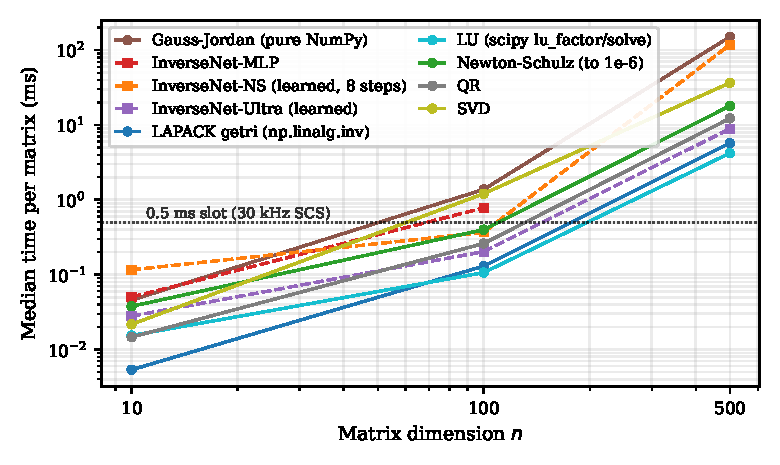
\includegraphics[width=0.82\textwidth]{figures/fig_time_vs_dim.pdf}
\caption{Median per-matrix inversion time versus dimension (log--log; CPU,
float32, batch size 1), generated from the verification rerun's raw
per-matrix results. Dashed lines with square markers are learned methods. The
dotted line marks the 0.5\,ms duration of a 5G NR slot at 30\,kHz subcarrier
spacing \cite{ts38211}, shown for interpretation only.}
\label{fig:time}
\end{figure}

\begin{figure}[t]
\centering
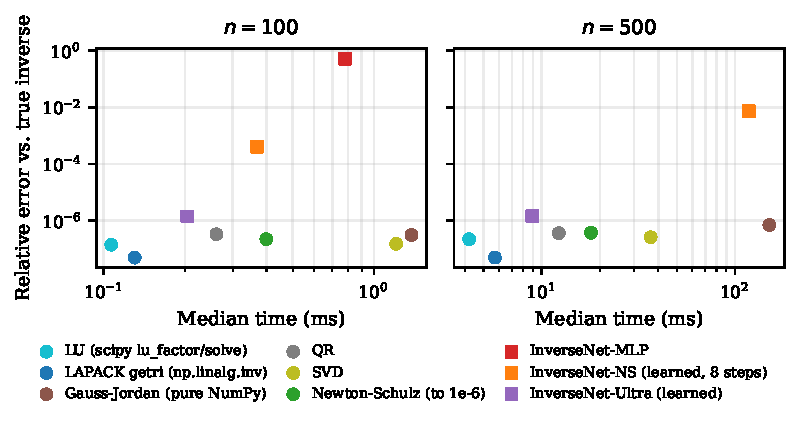
\includegraphics[width=0.9\textwidth]{figures/fig_accuracy_vs_time.pdf}
\caption{Latency--accuracy trade-off on the held-out set at $n{=}100$ (left)
and $n{=}500$ (right). Classical methods (circles) cluster at float32
machine-precision error; learned methods (squares) span six orders of
magnitude in error. InverseNet-MLP is absent at $n{=}500$ (infeasible).}
\label{fig:tradeoff}
\end{figure}

Table~\ref{tab:results} and Figures~\ref{fig:time}--\ref{fig:tradeoff}
support five findings.

\textbf{(F1) LAPACK-backed LU inversion is the reference to beat at every
size.} The two LU routes --- \texttt{numpy.linalg.inv} (getri) and SciPy's
\texttt{lu\_factor}/\texttt{lu\_solve} --- are the fastest accurate methods,
with medians of 0.005--0.015\,ms ($n{=}10$), 0.11--0.13\,ms ($n{=}100$), and
4.2--5.7\,ms ($n{=}500$), at float32 machine-precision error. QR costs about
$2\times$ and SVD $6$--$9\times$ the getri median at $n\!\ge\!100$ with no
accuracy benefit on these well-conditioned inputs, and the pure-NumPy
Gauss--Jordan implementation, dominated by its per-pivot Python loop, is
$26\times$ slower at $n{=}500$ (150.3 vs.\ 5.7\,ms) --- library routines win.

\textbf{(F2) Direct regression of the inverse fails.} InverseNet-MLP trains
to low loss but its held-out relative error is 0.36 ($n{=}10$) and 0.52
($n{=}100$): the output is unusable as an inverse, and the architecture cannot
represent $n{=}500$ at all. Learning the map $A \mapsto A^{-1}$ end-to-end,
without algorithmic structure, did not generalize from 800 training samples.

\textbf{(F3) Keeping the algorithmic structure helps, but is not uniformly
reliable.} The unrolled InverseNet-NS reaches $4.0\times10^{-4}$ relative
error at $n{=}100$, consistent with the premise of algorithm unrolling
\cite{monga2021unrolling}; yet the same 8-step recipe gives only
$4.0\times10^{-2}$ at $n{=}10$ and $7.3\times10^{-3}$ at $n{=}500$.
InverseNet-Ultra attains $1.4\times10^{-6}$ at $n{=}100$ and $n{=}500$ but
\emph{fails} at $n{=}10$ ($1.7\times10^{-1}$), indicating that its learned
initialization does not transfer across dimensions. Per-dimension tuning
remains necessary, and no learned model reaches classical accuracy.

\textbf{(F4) On CPU, no learned method beats the LAPACK baseline at the
median.} InverseNet-Ultra is the fastest learned model (0.204\,ms at
$n{=}100$; 8.92\,ms at $n{=}500$, timed through its NumPy/BLAS path) but is
still about $1.6\times$ slower than \texttt{getri} at the median at both
sizes. We note a timing caveat: the Ultra model runs through a NumPy
inference engine while MLP/NS run through PyTorch, so learned-vs-learned
latency comparisons mix runtimes; the learned-vs-LAPACK conclusion is
unaffected.

\textbf{(F5) Latency predictability depends on the implementation path;
fixed-step methods are uniformly predictable but not faster.} Because the
unrolled models execute a fixed number of matrix multiplies, their latency is
nearly deterministic in both runs (p95/median $\le 1.1$ everywhere, e.g.\
InverseNet-NS at $n{=}500$: $123.9/117.8 = 1.05$). Among the classical
routines, \texttt{getri} was equally flat on the lightly loaded host
(p95/median $= 1.04$ at $n{=}500$) but its median tripled under the archived
run's thread oversubscription, and the SciPy LU and QR calls showed strongly
bimodal latency even on the quiet host (scipy-LU at $n{=}500$: median
4.2\,ms, p95 110.0\,ms). For deadline-scheduled DU pipelines this means the
attractive scipy-LU median is not dependable without core pinning and BLAS
thread control, whereas the fixed-step methods' cost is stable but higher.

\textbf{Interpretation for fronthaul load management.} Reading
Figure~\ref{fig:time} against the 0.5\,ms slot at 30\,kHz subcarrier spacing
\cite{ts38211}: per-slot re-inversion of an $n{=}100$ matrix
(massive-MIMO covariance scale) costs ${\sim}0.13$\,ms at the median on a
plain CPU core and fits the slot with margin, whereas $n{=}500$ costs
${\sim}5.7$\,ms (and $3\times$ that under host contention) and cannot be
refreshed per slot on this class of hardware ---
such matrices must be updated at channel-coherence cadence, tracked
incrementally, or offloaded to an accelerator. These are compute-time
statements under our protocol (single core, Python-driven calls, batch size
1), not end-to-end latency claims.

\subsection{Current status and prior exploratory phase}

Classifying the project's components by evidence: \emph{(implemented and
evaluated)} the full inversion benchmark above, whose dataset, code, models,
raw results, and a September 2026 verification rerun all agree; \emph{(implemented but not
independently verifiable)} an earlier exploratory study of IQ-compression
encoders (O-RAN-style BFP and truncated-SVD baselines plus two custom
encoders), for which experiment drivers and result figures are preserved in
the repository but whose core source package (\texttt{src/}) was never
committed --- its numerical claims are therefore excluded from this report's
findings, and restoring that package is the first item of planned work;
\emph{(designed only)} a deadline-aware capacity-allocation controller for
multiple cells sharing one fronthaul link, for which a design document exists
but no implementation or results, scheduled next (Section~\ref{sec:plan}).

\subsection{Limitations}

(i)~Test matrices are synthetic, real-valued, and well conditioned by
construction; complex-valued, possibly ill-conditioned channel/covariance
matrices from a standardized channel model may reorder the accuracy results,
particularly for the iterative methods. (ii)~Timings are Python-driven,
CPU-only, batch size 1 on a shared machine; they upper-bound optimized
implementations, and BLAS thread contention inflates tail statistics
(e.g.\ scipy-LU at $n{=}500$: mean 20.6\,ms vs.\ median 4.2\,ms in the
rerun). (iii)~The learned models' expected advantage --- batched inference on
GPU/NPU hardware --- is an untested hypothesis here, not a result.
(iv)~Prediction accuracy of an inverse does not by itself establish
link-level benefit (e.g.\ precoding quality); coupling these costs to a
fronthaul simulation remains future work. (v)~The $10^{-3}$--$10^{-6}$ errors
of the learned methods, while orders of magnitude better than direct
regression, have not been mapped to an acceptable equalization/precoding
error budget.

% ===================== SECTION 5 =====================
\section{Planned Workflow and Timeline}
\label{sec:plan}

The plan below is driven by the demonstrated gaps: the unverifiable
compression phase, the missing complex-channel evaluation, and the
design-only allocation controller. The end-semester evaluation (ESE) is
expected in the last week of November 2026 (date to be confirmed).

\begin{table}[h]
\centering
\small
\caption{Planned workflow from the report date to the expected ESE period.}
\label{tab:plan}
\begin{tabular}{@{}p{2.6cm} p{5.7cm} p{4.6cm} p{2.6cm}@{}}
\toprule
Target window & Task & Deliverable / success criterion & Depends on \\
\midrule
Late Sep--early Oct & Restore/reimplement the compression \texttt{src/} package; re-run its four experiments & Compression results reproduced from committed code, or revised & --- \\
Mid Oct & Extend benchmark to complex-valued channel-model matrices; pinned-core and batched timing & Benchmark v2 with Hermitian solves; tail statistics under pinning & Benchmark (done) \\
Late Oct--mid Nov & Implement the multi-cell fronthaul capacity-allocation simulator (queues, deadlines, budget controllers) and baseline policies & Working simulator; baseline comparison on seeded synthetic traffic & Design doc; benchmark cost model \\
Mid--late Nov & Integrate compression setting $\leftrightarrow$ offered load $\leftrightarrow$ allocation; ESE report and presentation; supervisor review; authorized similarity check & ESE-ready report and defended results & All above \\
\bottomrule
\end{tabular}
\end{table}

\textbf{Progress summary.} The measurement layer of the project is complete
and verified: a seeded, reproducible benchmark establishing that (a) tuned
LAPACK inversion is the CPU reference at all tested sizes, (b) structure-free
learned inversion fails while unrolled-iteration models are accurate to
$10^{-4}$--$10^{-6}$ at $n \ge 100$ with dimension-dependent failure cases, and
(c) fixed-step methods offer predictable latency rather than lower median
latency. \textbf{Next technical milestone:} a re-runnable compression
result set (restored \texttt{src/}), followed by the allocation simulator
that consumes both the compression operating points and the compute budgets
measured here.

% ===================== REFERENCES =====================
\begin{thebibliography}{9}
\setlength{\itemsep}{1pt}\small

\bibitem{larsen2019survey}
L.~M.~P. Larsen, A.~Checko, and H.~L. Christiansen, ``A survey of the
functional splits proposed for 5G mobile crosshaul networks,'' \emph{IEEE
Communications Surveys \& Tutorials}, vol.~21, no.~1, pp. 146--172, 2019,
doi: 10.1109/COMST.2018.2868805.

\bibitem{polese2023oran}
M.~Polese, L.~Bonati, S.~D'Oro, S.~Basagni, and T.~Melodia, ``Understanding
O-RAN: Architecture, interfaces, algorithms, security, and research
challenges,'' \emph{IEEE Communications Surveys \& Tutorials}, vol.~25,
no.~2, pp. 1376--1411, 2023, doi: 10.1109/COMST.2023.3239220.

\bibitem{oran_cus}
O-RAN Alliance Working Group 4, ``Control, user and synchronization plane
specification,'' O-RAN.WG4.CUS.0, technical specification (open fronthaul
interface).

\bibitem{wu2014mimo}
M.~Wu, B.~Yin, G.~Wang, C.~Dick, J.~R. Cavallaro, and C.~Studer,
``Large-scale MIMO detection for 3GPP LTE: Algorithms and FPGA
implementations,'' \emph{IEEE Journal of Selected Topics in Signal
Processing}, vol.~8, no.~5, pp. 916--929, Oct. 2014, doi:
10.1109/JSTSP.2014.2313021.

\bibitem{schulz1933}
G.~Schulz, ``Iterative Berechnung der reziproken Matrix,'' \emph{Zeitschrift
f\"ur Angewandte Mathematik und Mechanik}, vol.~13, no.~1, pp. 57--59, 1933,
doi: 10.1002/zamm.19330130111.

\bibitem{gregor2010lista}
K.~Gregor and Y.~LeCun, ``Learning fast approximations of sparse coding,'' in
\emph{Proc. 27th International Conference on Machine Learning (ICML)}, Haifa,
Israel, 2010, pp. 399--406.

\bibitem{monga2021unrolling}
V.~Monga, Y.~Li, and Y.~C. Eldar, ``Algorithm unrolling: Interpretable,
efficient deep learning for signal and image processing,'' \emph{IEEE Signal
Processing Magazine}, vol.~38, no.~2, pp. 18--44, Mar. 2021, doi:
10.1109/MSP.2020.3016905.

\bibitem{ts38211}
3GPP, ``NR; Physical channels and modulation,'' Technical Specification TS
38.211 (Release 15 onward).

\end{thebibliography}

\end{document}
